%12/02 - Modesto
\chapter{Modelado por homología}
\section{Modelización de estructuras proteicas: Cuidado con las diferencias}
El número de secuencias de proteínas en las bases de datos ha crecido exponencialmente en las últimas décadas, sobre todo tras la revolución de los métodos de secuenciación de alto rendimiento.

Sin embargo, la determinación experimental de estructuras tridimensionales de proteínas suele ser difícil, requiere mucho tiempo y está sujeta a limitaciones, como los errores experimentales, la interpretación de los datos y la modelización de nuevos datos sobre estructuras ya publicadas. Así, a pesar de los considerables esfuerzos iniciados a principios del siglo XXI para aplicar métodos de biología estructural de alto rendimiento, la disponibilidad de estructuras de proteínas es más de 1.000 veces inferior al número de secuencias. Por ejemplo, en febrero de 2025, hay ,más de 250 M de secuencias en Uniprot o más de 700 M de proteínas en MGnify, mientras que sólo alrededor de 220k estructuras en RCSB Protein Databank. Esta diferencia se denomina brecha secuencia-estructura de proteínas y se amplía constantemente, especialmente si consideramos las secuencias de las bases de datos de metagenómica no disponibles en Uniprot.

Así pues, para compensar la falta de datos experimentales es necesario predecir con precisión y fiabilidad la estructura tridimensional de una proteína determinada.

\section{¿Son predecibles las estructuras de las proteínas?}
Las propiedades de los aminoácidos determinan los ángulos $\Phi$ y $\Psi$ que acaban conformando los niveles estructurales superiores. Sin embargo, el plegamiento de proteínas puede ser más complejo, ya que debe acoplarse a la síntesis de proteínas.

Cabe imaginar que la complejidad y diversidad de las estructuras proteicas en la naturaleza puede ser enorme. De hecho, John Kendrew y sus colaboradores parecían muy decepcionados por la determinación de la primera estructura globular tridimensional, la mioglobina en 1958:
\begin{quote}
Quizá las características más notables de la molécula sean su complejidad y su falta de simetría. La disposición parece carecer casi por completo del tipo de regularidades que uno anticipa instintivamente, y es más complicada de lo que ha anticipado cualquier teoría de la estructura de las proteínas.
\end{quote}

No mucho más tarde, en 1968, Cyrus Levinthal (1922-1990) publicó la llamada paradoja de Levinthal, afirmando que las proteínas se pliegan en nano/milisegundos, pero incluso para los péptidos pequeños llevará un tiempo enorme probar el astronómico número de conformaciones posibles. Digamos que una proteína pequeña de 100 aminoácidos tiene 99 enlaces peptídicos y 198 ángulos $\Phi$ y $\Psi$ diferentes. Suponiendo sólo 3 conformaciones alternativas para cada enlace, se obtendrán $3^{198} (= 2,95 \times 10^{95})$ conformaciones posibles. Si diseñamos un algoritmo altamente eficiente que pruebe 1 conformación por nanosegundo:
$$2.95 \times 10^{85} \text{segundos} = 9 \times 10^{67} \text{mil millones de años}$$
Teniendo en cuenta que la edad del universo es de 13.800 millones de años, predecir las estructuras de las proteínas no parece tarea fácil.

En este contexto, un experimento muy sencillo realizado hace 50 años arrojó algo de luz sobre el mecanismo de plegamiento de las proteínas. Cristian Anfisen fue capaz de desnaturalizar (desdoblar) completamente la Ribonucleasa A, mediante la adición de agentes reductores y urea bajo tratamiento térmico, y posteriormente cambiar a condiciones normales que permiten a la proteína volver a plegarse de forma totalmente funcional. Este experimento indica que la secuencia de aminoácidos dicta la estructura final. A pesar de algunas excepciones relevantes, esto se ha confirmado en gran medida.
\begin{figure}[h]
\centering
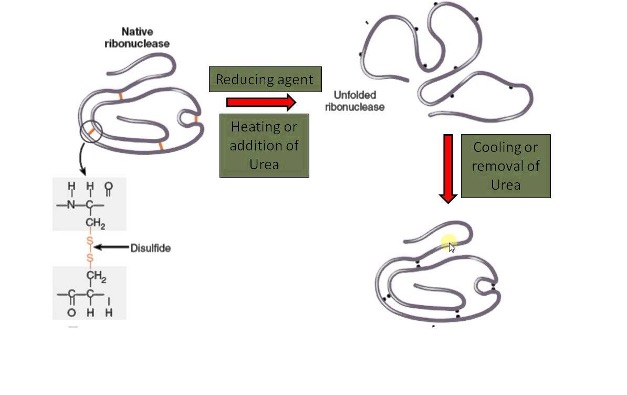
\includegraphics[width = 0.8\textwidth]{figs/anfinsen.jpg}
\caption{El dogma de Anfinsen: La secuencia de aminoácidos dictaba la estructura final. }
\end{figure}

Cabe imaginar que las estructuras nativas in vivo de las proteínas se parecen a la conformación más estable, es decir, al mínimo global de energía libre. Ésa es la base del modelo de embudo del plegamiento de proteínas, que supone que el número de conformaciones posibles se reduce cuando se alcanza un mínimo local de energía, lo que constituye un camino para el proceso de plegamiento.
\begin{figure}[h]
\centering
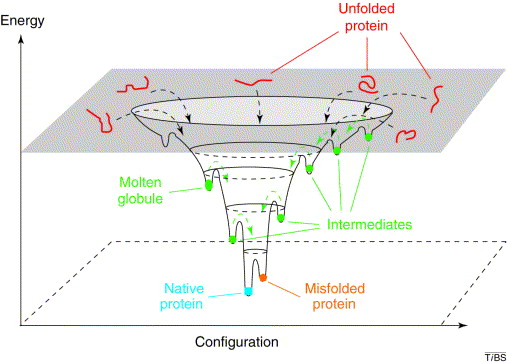
\includegraphics[width = 0.8\textwidth]{figs/funnel_1.jpeg}
\caption{Diagrama esquemático del paisaje energético de plegamiento de una proteína según el modelo del embudo. Las moléculas desnaturalizadas situadas en la parte superior del embudo pueden plegarse al estado nativo por una miríada de rutas diferentes, algunas de las cuales implican intermedios transitorios (mínimos energéticos locales), mientras que otras implican trampas cinéticas significativas (estados mal plegados).}
\end{figure}

\begin{table}[htbp]
\begin{mdframed}[backgroundcolor=black!10]
    \centering
    \textbf{Conclusión}: Se pueden predecir las estructuras de las proteínas porque sólo dependen de su secuencia. Pero para obtener predicciones precisas, o bien se necesita mucho tiempo y potentes ordenadores... o métodos realmente eficaces. 
    \end{mdframed}
\end{table}

El \textbf{modelado por homología} es uno de los trucos más convenientes para sortear esta limitación. Básicamente, la estrategia consiste en añadir más capas de información adicional a las propiedades de los aminoácidos, a saber, la conservación evolutiva de secuencias y estructuras.

Muy a menudo, antes de crear los modelos ya se dispone de cierta información sobre la proteína. Por ejemplo, si se trata de una enzima, es posible que se hayan descubierto los residuos catalíticos o la región de interacción con el sustrato. También es aconsejable buscar en la literatura, en particular para ver si hay un artículo complementario de la(s) estructura(s) PDB correspondiente(s) que pueda estar disponible o que pueda encontrar y utilizar como plantilla(s) para el modelado.

\section{Modelización comparativa: La conservación es la clave}
\begin{figure}[h]
\centering
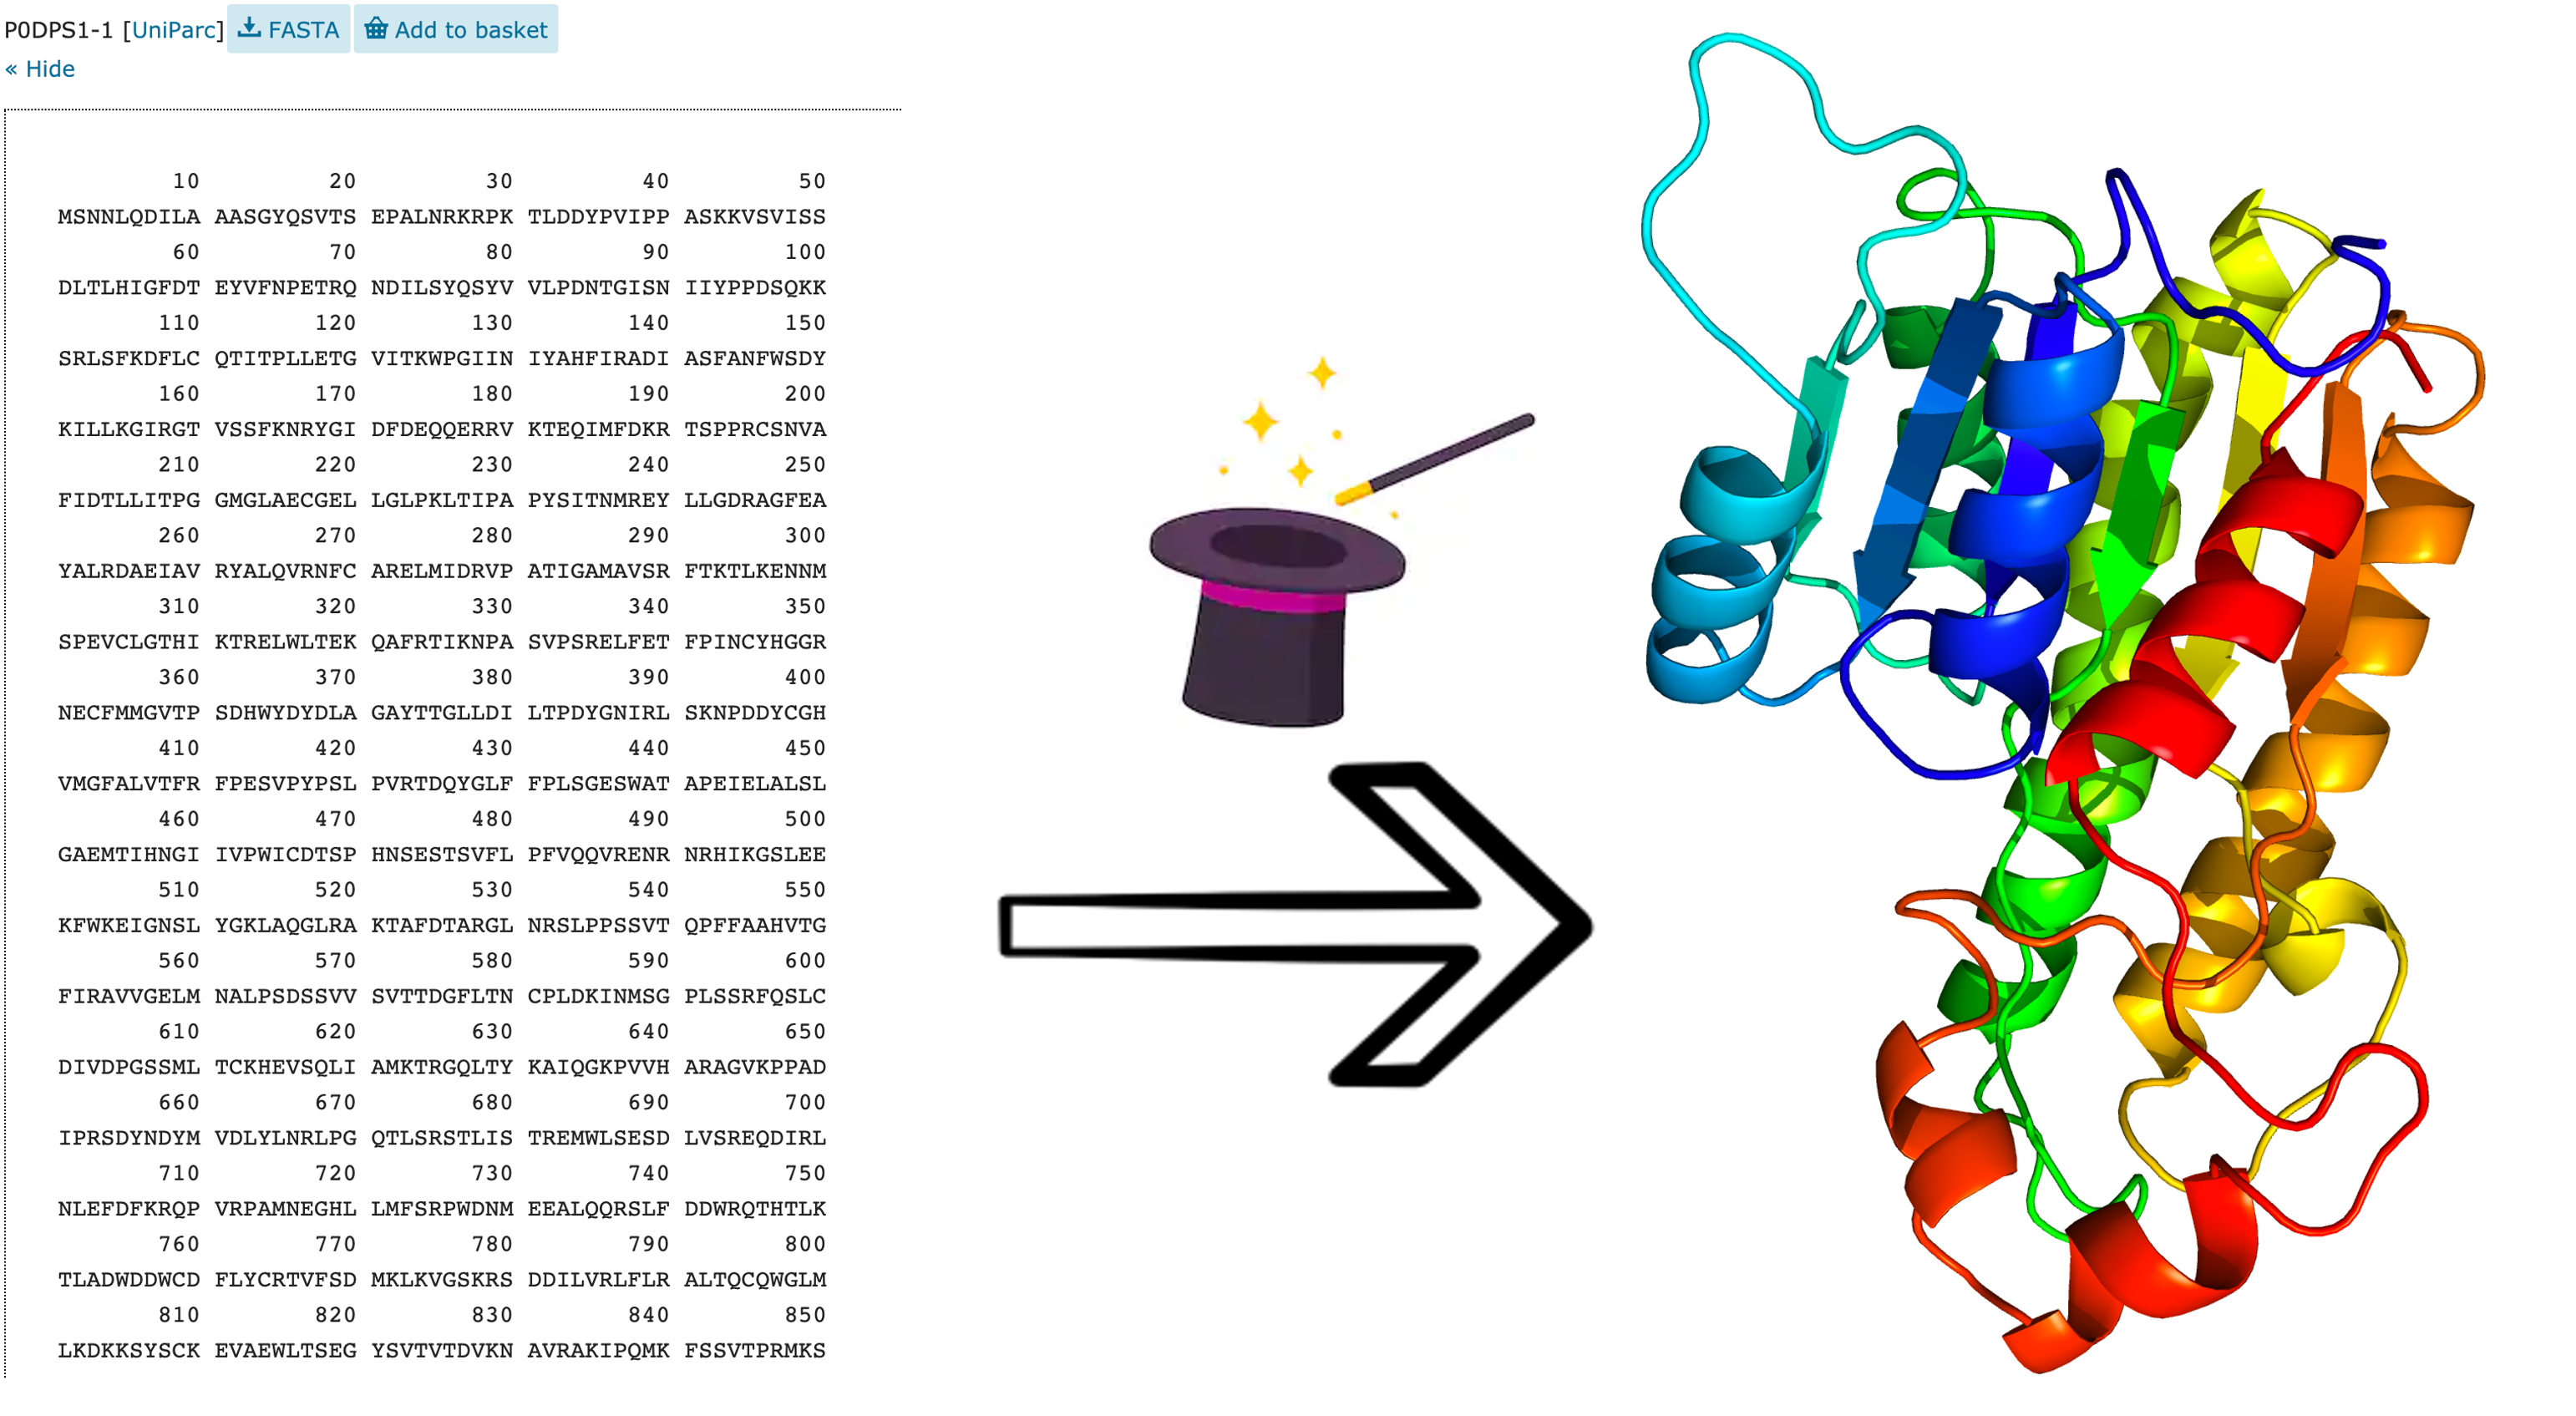
\includegraphics[width = 0.7\textwidth]{figs/modeling.png}
\caption{En pocas palabras, el modelado de proteínas consiste en pasar de la secuencia a la estructura. Pero, ¿cómo lo hacemos?}
\end{figure}

Tradicional y conceptualmente, la predicción de la estructura de las proteínas puede abordarse desde dos perspectivas diferentes: el modelado comparativo y la predicción \textit{ab initio}. En el enfoque del modelado comparativo, sólo se puede predecir la estructura tridimensional de secuencias de proteínas si se encuentran sus homólogas en la base de datos de proteínas con estructuras conocidas. Por supuesto, la identificación de tales homólogos es clave en este caso. Hasta hace poco, la mayor parte del desarrollo en el modelado de proteínas ha estado impulsado por el desarrollo de métodos para identificar similitudes de secuencias distantes que reflejarían pliegues proteicos similares. Por otra parte, el modelado \textit{ab initio} se basa únicamente en las propiedades fisicoquímicas de la molécula.

\begin{table}[htbp]
\begin{mdframed}[backgroundcolor=black!10]
    \centering
    Los términos «modelización homológica» y «modelización comparativa» suelen utilizarse indistintamente. Sin embargo, el modelado comparativo puede considerarse un enfoque más amplio que aprovecha las estructuras conocidas y abarca tanto el modelado homológico como el reconocimiento de pliegues o el enhebrado.
    \end{mdframed}
\end{table}

\begin{figure}[h]
\centering
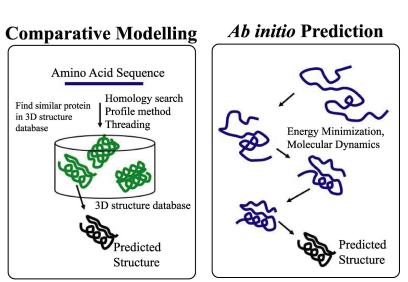
\includegraphics[width = 0.5\textwidth]{figs/predway.jpeg}
\caption{Dos enfoques diferentes para la predicción de estructuras.}
\end{figure}

El modelado homológico genera modelos estructurales basados en la estructura de (normalmente) una estructura homóloga relacionada. Así pues, la precisión del modelado homológico está limitada por la disponibilidad de estructuras similares. Las predicciones \textit{ab initio} están limitadas por los modelos matemáticos y los recursos informáticos, y a menudo sólo son útiles para péptidos pequeños.

Para mantener la estructura y la función, determinados aminoácidos de la secuencia proteica están sometidos a una mayor presión de selección. O bien evolucionan más despacio de lo esperado o dentro de ciertas restricciones, como la similitud química (es decir, sustituciones conservadoras). Por lo tanto, los enfoques de modelado homológico asumen que una secuencia proteica similar implica una estructura 3D y una función similares. De hecho, las proteínas en la naturaleza no parecen contener toda la diversidad posible. Así, aunque el número de secuencias y estructuras publicadas aumenta constantemente, el número de pliegues únicos se mantuvo casi constante desde 2008 hasta hace muy poco.

Esto significa que el espacio de secuencias de proteínas es mucho mayor que el espacio de estructuras. Algunas bases de datos, como Scop2 o CATH (Figura \ref{fig:cath}) han aprovechado esta circunstancia empleando clasificaciones jerárquicas de estructuras en un número limitado de categorías distintas. Entre 2006 y 2024, el número de dominios diferentes en CATH aumentó de 86.000 a 600.000, mientras que el número de arquitecturas se mantuvo relativamente estable en 40 y 43, respectivamente. Incluso después de analizar numerosas estructuras nuevas de la base de datos AlphaFold, sólo se identificaron 25 superfamilias nuevas (y ninguna arquitectura nueva) (Figura \ref{fig:cath2}).

\begin{figure}[h]
\centering
\includegraphics[width = 0.5\textwidth]{figs/cath.png}
\caption{Ejemplificaciones de las principales categorías de CATH en 2006.}
\label{fig:cath}
\end{figure}

\begin{figure}[h]
\centering
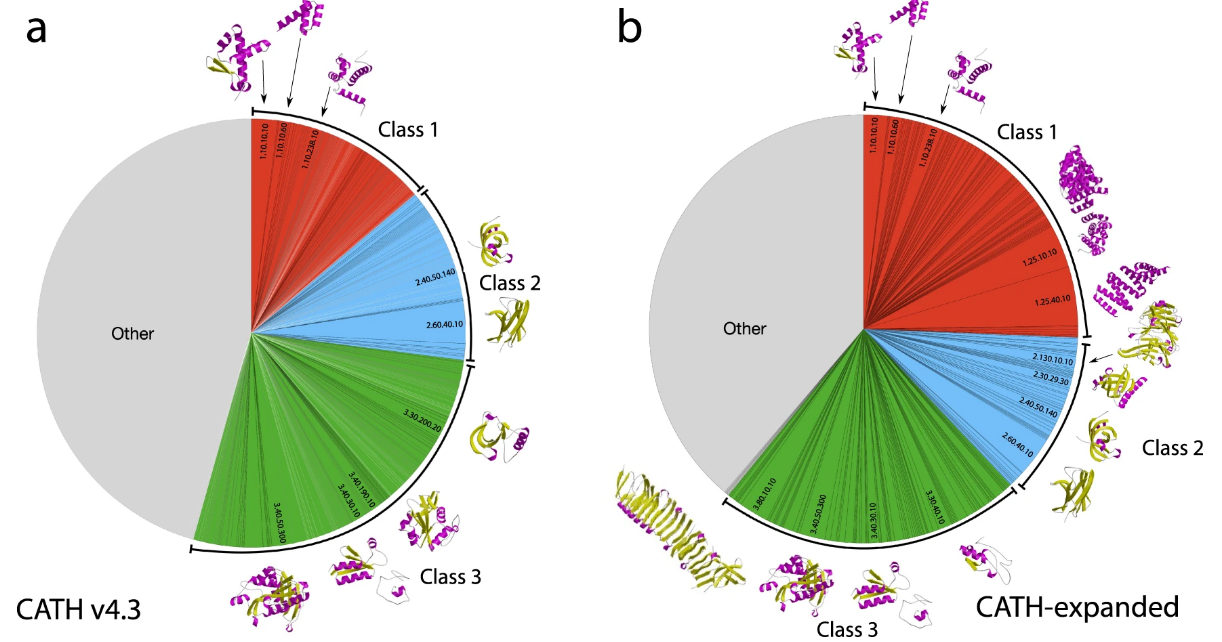
\includegraphics[width = 0.8\textwidth]{figs/cath2.png}
\caption{En 2022, la base de datos Alphafold amplió las principales categorías de CATH con 25 nuevas superfamilias.}
\label{fig:cath2}
\end{figure}

En resumen, las estructuras de las proteínas suelen estar más conservadas que sus secuencias, lo que permite construir modelos comparando proteínas con secuencias diferentes. Las secuencias biológicas evolucionan por mutación y selección, con una presión de selección variable para cada posición de residuo en una proteína en función de su importancia estructural y funcional. Los métodos de comparación de proteínas, como los alineamientos de secuencias, pretenden transmitir la historia evolutiva de las proteínas.

\section{Modelización homológica en cuatro pasos}
\begin{figure}[h]
\centering
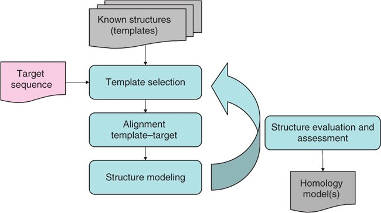
\includegraphics[width = 0.6\textwidth]{figs/homology_simple_workflow.png}
\caption{Flujo de trabajo del modelado de proteínas basado en una plantilla.}
\end{figure}

Un protocolo tradicional de modelización homológica construirá un modelo parcial o completo a partir de una secuencia de proeína basada en una única plantilla homóloga. En general, se requiere una identidad de secuencia mayor del 30\% entre la plantilla y la diana para obtener resultados fiables. Estos métodos requieren tres pasos (1) identificación de la plantilla más adecuada, (2) alineación de la secuencia de consulta y la plantilla, y (3) construcción del modelo. Estos pasos pueden abordarse con diferentes alternativas metodológicas y pueden arrojar diferentes resultados que deben evaluarse (paso 4) para encontrar la mejor solución para cada paso. 

En este curso, nos centraremos en el modelado de extremo a extremo utilizando SWISS-MODEL, un servidor de modelado totalmente automatizado que permite construir modelos sin necesidad de tener una sólida formación en bioinformática o conocimientos de programación. Las primeras versiones de SWISS-MODEL solo permitían el modelado de secuencias con homólogos en bases de datos, pero como se analiza a continuación, la implementación de avances en el reconocimiento de plantillas y la construcción de modelos ha aumentado la capacidad y la precisión del modelado, especialmente en los últimos 15 años.

SWISS-MODEL admite varias entradas. Normalmente, se introduce una consulta de secuencia única para la búsqueda de plantillas, pero también se puede omitir este paso e introducir directamente la plantilla deseada o incluso una plantilla y un alineamiento personalizado. Comenzaremos con la primera alternativa.

\subsection{Pasos 1 y 2: Búsqueda y alineación de plantillas}
\subsubsection{¿Dónde podemos buscar?}
La búsqueda de plantillas consiste en encontrar una proteína con estructura(s) conocida(s) con una secuencia relacionada con nuestra proteína. Como ya hemos mencionado, el Banco de Datos de Proteínas (PDB) del RCSB es la mayor base de datos de estructuras de proteínas. Así, podemos buscar plantillas comparando la secuencia de nuestra proteína con la secuencia de todas las proteínas del PDB. Sin embargo, el PDB se creó como repositorio para contener todas las estructuras macromoleculares, no para buscar plantillas para el modelado. Al igual que otros software de extremo a extremo, SWISS-MODEL tiene su propia base de datos curada, la SMLT (SWISS-MODEL template library). Se basa en alineaciones de perfiles del PDB, se actualiza semanalmente y también está anotada e indexada para facilitar la búsqueda. A día de 5 de febrero de 2025, SMLT contiene 158.703 secuencias de proteínas únicas que pueden mapearse en 386.135 unidades biológicas. Desde 2023, SWISS-MODEL también busca en la base de datos AlphaFold DB.

\subsubsection{¿Cómo podemos buscar de forma precisa y rápida?}
\begin{figure}[h]
\centering
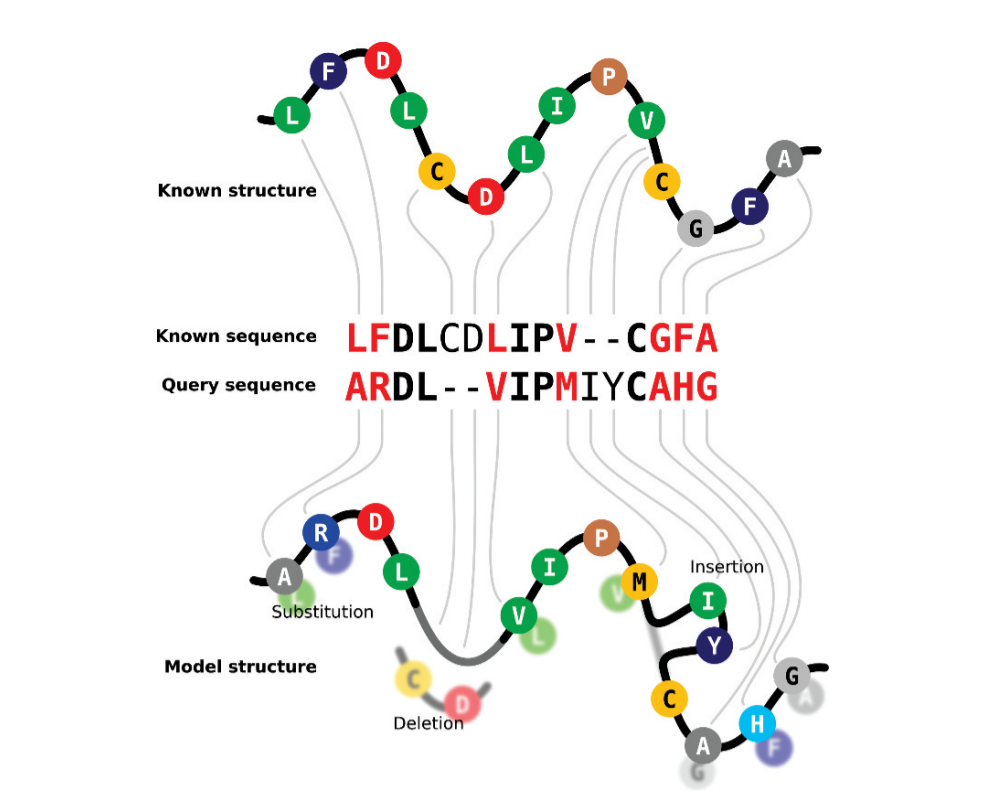
\includegraphics[width = 0.6\textwidth]{figs/template_query.png}
\caption{La alineación consulta-plantilla es la base del modelado homológico.}
\end{figure}

Para encontrar plantillas, hay que comparar secuencias, por lo que es esencial disponer de un método de alineación preciso y potente. Comparar la secuencia de una proteína con toda una base de datos lleva mucho tiempo porque se está comparando con proteínas completamente no relacionadas, lo que supone una pérdida de recursos. Dos mejoras fundamentales han aumentado la capacidad de búsqueda de plantillas: (1) la introducción de la estructura secundaria (SS) comparando las predicciones de SS de la proteína de consulta y las estructuras secundarias de la base de datos de proteínas, y (2) el uso de perfiles para facilitar la comparación. Los perfiles son un método matemático de resumir un alineamiento de secuencias múltiples que cuantifica la probabilidad de cada aminoácido en cada posición. Un tipo particular de perfil son los modelos de Markov ocultos (HMM), muy útiles para buscar secuencias similares en las bases de datos. También se modelan las probabilidades de transición (es decir, la probabilidad de que un aminoácido concreto siga a otro aminoácido concreto). 
Además, los HMM incluyen inserciones y deleciones de aminoácidos. Estas características permiten a los HMM modelar alineaciones enteras con gran detalle, incluidas regiones muy divergentes, y facilitan la identificación de posiciones muy conservadas que definen no sólo la función de las proteínas, sino también su plegamiento. Por ejemplo, residuos de glicina al final de cada cadena beta o un patrón de residuos polares que favorecen las hélices alfa. La comparación previa de la secuencia de consulta con una base de datos de secuencias nos permite incorporar información evolutiva sobre la secuencia. Así, pasamos de un requisito de más del 30\% de identidad para obtener buenos modelos antes de la implementación de perfiles, a buenos modelos incluso con $\sim$20\% de identidad o menos. Además, la generación de perfiles también facilita la agrupación de la base de datos de búsqueda, reduciendo el tiempo de búsqueda. La implementación de estas capacidades condujo a la implementación del llamado reconocimiento de pliegues en el modelado homológico.

\begin{figure}[h]
\centering
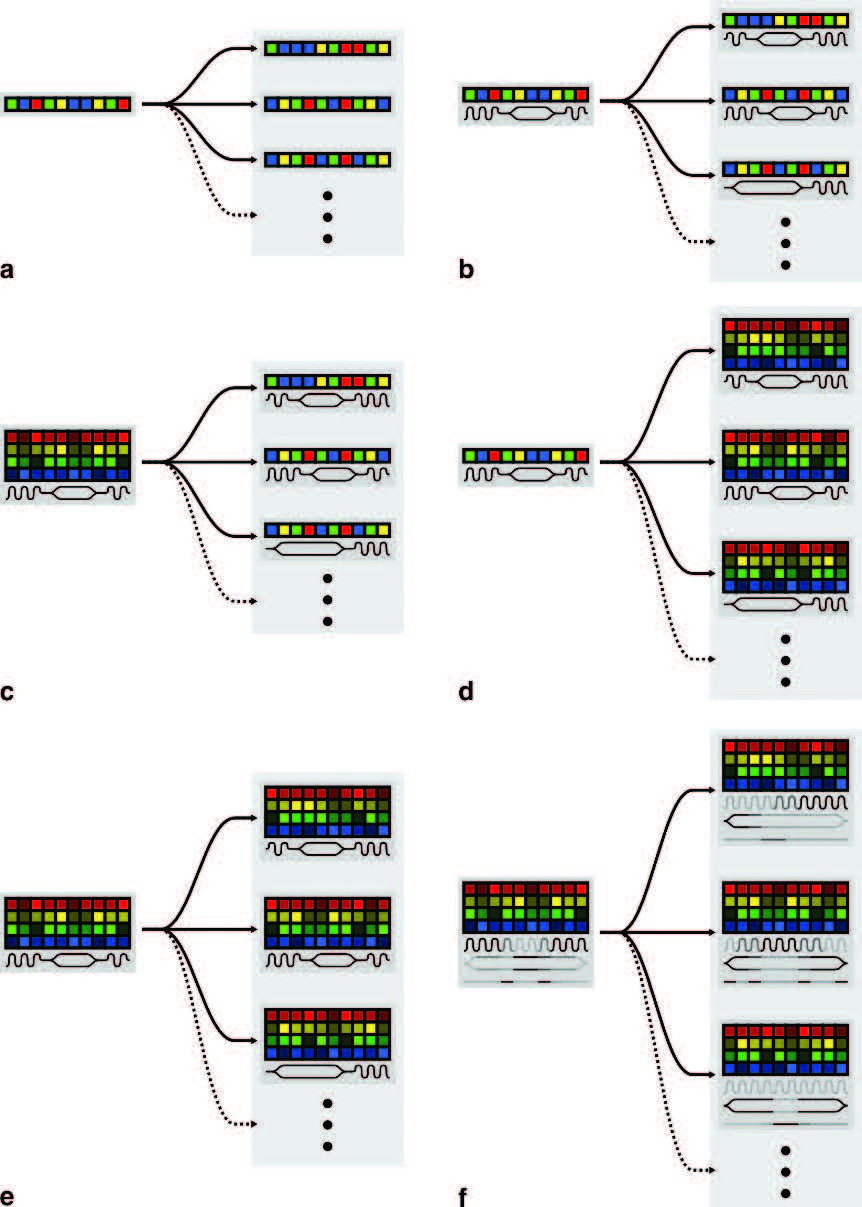
\includegraphics[width = 0.6\textwidth]{figs/profiles.jpg}
\caption{De la búsqueda secuencia contra secuencia a la comparación perfil-perfil.}
\end{figure}

La búsqueda de plantillas en SWISS-MODEL ha evolucionado a lo largo de los años hacia resultados más precisos. Actualmente, se realiza con \textbf{HHblits}, un método iterativo de perfil-perfil. También podemos buscar plantillas utilizando Blast u otros métodos de perfil-perfil, como Psi-BLAST, HHPred o JackHMMER. A continuación, las plantillas se clasifican entre 0 y 1 utilizando dos parámetros numéricos diferentes: \textbf{GMQE} (estimación global de la calidad del modelo) y \textbf{QSQE} (estimación de la calidad de la estructura cuaternaria). Brevemente, GMQE utiliza funciones de verosimilitud para evaluar varias propiedades de la alineación diana-plantilla (identidad de secuencia, similitud de secuencia, puntuación HHblits, concordancia entre la estructura secundaria predicha de la diana y la plantilla, concordancia entre la accesibilidad al disolvente predicha entre la diana y la plantilla; todo ello normalizado por la longitud de la alineación) para predecir la calidad esperada del modelo resultante. QSQE evalúa la probabilidad del estado oligomérico del modelo.

\subsection{Paso 3: Construcción del modelo}
Por defecto, SWISS-MODEL proporcionará 50 posibles plantillas clasificadas. La salida también contiene información sobre el método y la resolución de las plantillas, el porcentaje de identidad (y la cobertura de la alineación) con la secuencia de consulta, y el GMQE y QSQE.

La plantilla superior está marcada por defecto y es probable que dé el mejor modelo, pero también es interesante probar algunas plantillas alternativas dependiendo de la aplicación posterior del modelo. Por ejemplo, con un sustrato/cofactor diferente que pueda tener un papel clave en la función de la proteína o con una cobertura o porcentaje de identidad diferente.

Una vez seleccionada(s) la(s) plantilla(s), se construyen las coordenadas del modelo basándose en la alineación de la secuencia de consulta y de la plantilla utilizando el módulo ProMod3. SWISS-MODEL utiliza un ensamblaje de fragmentos, que es también la base de los métodos Fold-recognition o Threading. Otros programas, como Modeller, se basan en la satisfacción de restricciones espaciales generales. Modeller es una herramienta de línea de comandos que permite la personalización completa del modelado, lo que requiere más conocimientos sobre el proceso pero puede ser muy útil para algunos tipos de proteínas. No obstante, se ha implementado en algunos servidores en línea (ModWeb), cuadernos de Python y aplicaciones de fácil uso, como ChimeraX y Pymol (plugin Pymod). Modeller también se puede llamar desde la salida de HHPred (si se incluyó PDB como base de datos de búsqueda), lo que es muy conveniente para modelar homólogos remotos utilizando varias plantillas en pocos minutos.

El ensamblaje de fragmentos utilizará los átomos de la columna vertebral del núcleo de la plantilla para construir una estructura central del modelo, dejando las regiones no conservadas (principalmente bucles) para más adelante. El \textbf{modelado de bucles} incluye el uso de un subconjunto de homólogos de una base de datos de bucles específica, el muestreo de Monte Carlo como alternativa e incluso la construcción \textit{ab initio} de bucles que faltan.

\begin{figure}[h]
\centering
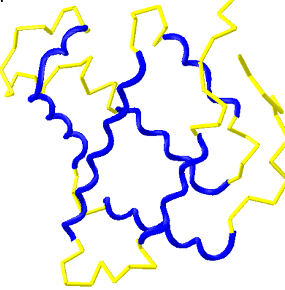
\includegraphics[width = 0.4\textwidth]{figs/loops.png}
\caption{Modelado de backbone y loop.}
\end{figure}

A continuación, se procede al posicionamiento de la \textbf{cadena lateral} de los aminoácidos no conservados. El objetivo es encontrar la conformación más probable de la cadena lateral, utilizando la información de la estructura plantilla, las bibliotecas de rotámeros (de un conjunto curado de estructuras de proteínas conocidas) y criterios energéticos y de empaquetamiento. Si hay que colocar muchas cadenas laterales en la estructura, se producirá el «problema del huevo y la gallina», ya que la colocación de un rotámero afectaría a los demás. Eso significa que la identificación de posibles enlaces de hidrógeno entre las cadenas laterales de los residuos y entre las cadenas laterales y la columna vertebral reduce los cálculos de optimización. Al fin y al cabo, cuantos más residuos se posicionen correctamente, mejor será el modelo.

\begin{figure}[h]
\centering
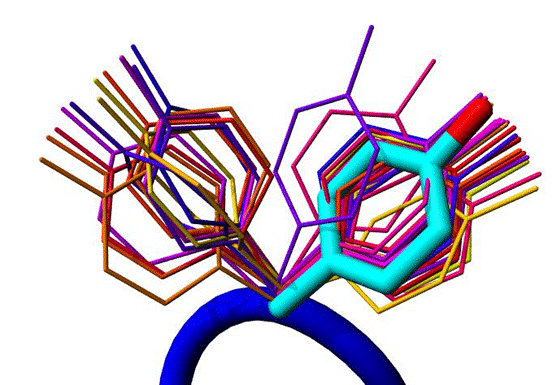
\includegraphics[width = 0.5\textwidth]{figs/Rotamers.png}
\caption{Modelado de cadena lateral.}
\end{figure}

Por último, se lleva a cabo una breve minimización de la energía para reducir los contactos y enlaces desfavorables adaptando las geometrías angulares y relajando los contactos cercanos. Este paso de minimización de energía o refinamiento puede ser útil para conseguir mejores modelos, pero sólo cuando el plegamiento ya es preciso.

\subsection{Paso 4: Evaluación de resultados}
El ordenador siempre te da un modelo, pero eso no significa que tenga un modelo que tenga sentido. ¿Cómo podemos saber si podemos fiarnos del modelo? Los modelos de salida están coloreados en una escala de colores de temperatura, del azul marino (buena calidad) al rojo (mala calidad). Eso puede ayudarnos a entender nuestro modelo a primera vista. Además, se trata de un sitio interactivo y se puede acercar y alejar el modelo. Hay muchas otras funciones disponibles para trabajar en tu modelo. Por ejemplo, puedes comparar varios modelos, puedes cambiar las opciones de visualización. También puedes descargar todos los archivos e informes en el botón «Datos del proyecto».

También existe la opción «Evaluación de la estructura». Esta opción proporciona un informe detallado de los problemas estructurales de su modelo. Se pueden ver gráficos de Ramachandran que resaltan en rojo los residuos de aminoácidos con ángulos phi/psi anormales en el modelo y una lista detallada de otros problemas.

El GMQE se actualiza con la puntuación QMEAN Z y QMEANDisCo (Studer et al. 2020). La puntuación QMEAN Z o la puntuación QMEAN normalizada indica cómo se compara el modelo con estructuras experimentales de tamaño similar. Una puntuación QMEAN Z en torno a 0 indica una buena concordancia, mientras que las puntuaciones por debajo de -4,0 se dan a modelos de baja calidad. Además del número, un gráfico muestra la puntuación QMEAN de nuestro modelo (estrella roja) dentro de todas las puntuaciones QMEAN de estructuras determinadas experimentalmente en comparación con su tamaño. En general, la puntuación Z equivale a la desviación estándar de la media.

\begin{figure}[h]
\centering
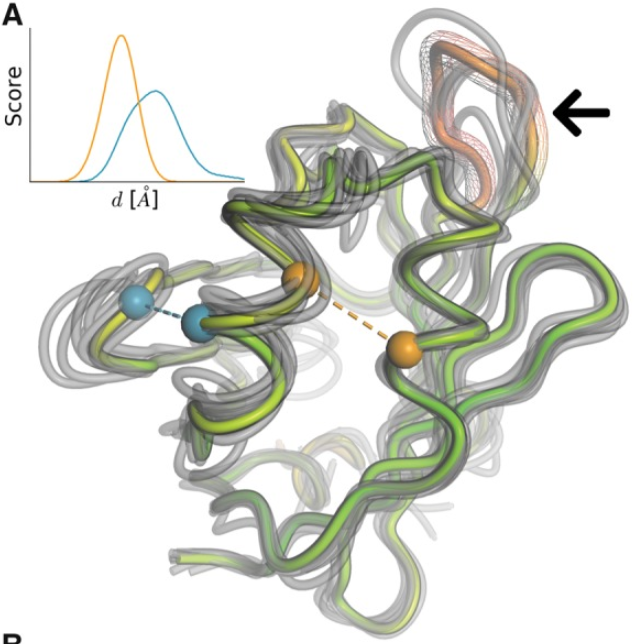
\includegraphics[width = 0.5\textwidth]{figs/paste-C2BED0C6.png}
\caption{Las puntuaciones QMEANDisCo por residuo se representan como un gradiente de color rojo a verde en un modelo de lbp-8 en \textit{Caenorhabditis elegans} (UniProtKB: O02324, PDB: 6C1Z). Las restricciones de distancia se han construido a partir de un conjunto de estructuras proteicas determinadas experimentalmente que son homólogas a lbp-8. El recuadro muestra dos ejemplos de restricciones entre residuos marcados con esferas de colores en el modelo. }
\end{figure}

El QMEANDisCO se implementó en SWISS-MODEL en 2020 y es un potente parámetro único que combina potenciales estadísticos y términos de acuerdo con una restricción de distancia (DisCo) para proporcionar una puntuación de consenso. DisCo evalúa la consistencia de las distancias CA-CA por pares de un modelo con restricciones extraídas de estructuras homólogas. Todas las puntuaciones se combinan utilizando una red neuronal entrenada para predecir puntuaciones por residuo. Podemos comprobar una puntuación global, pero también una puntuación local para cada residuo, que nos ayudan a comprender qué regiones del modelo tienen más probabilidades de plegarse con precisión (es decir, son más fiables).

\href{https://swissmodel.expasy.org/assess}{Swissmodel Assessment} también se puede utilizar como herramienta externa para analizar modelos obtenidos con otros métodos con el fin de hacerlos comparables, sólo necesita archivos .pdb de su modelo y, opcionalmente, la proteína modelo de referencia.

Existen otras herramientas independientes de evaluación de modelos que se utilizan habitualmente para evaluar modelos de proteínas, como VoroMQA o MoldFold. VoroMQA es un método muy rápido que combina la idea de potenciales estadísticos (es decir, una función de puntuación basada en el conocimiento) con el uso de áreas de contacto interatómico para proporcionar una puntuación en el rango de [0,1]. Cuando se aplica a la base de datos PDB, la mayoría de las estructuras de alta calidad basadas en experimentos tienen una puntuación VoroMQA >0,4. Por lo tanto, si la puntuación es superior a 0,4, es probable que el modelo sea bueno y los modelos con una puntuación <0,3 son probablemente malos. Los modelos con una puntuación de 0,3-0,4 son inciertos y no deben clasificarse con VoroMQA. Por otro lado, ModFold es una metaherramienta que le proporciona un informe muy detallado (y archivos parseables) con puntuaciones locales y globales, pero puede tardar horas/días en obtener el resultado, por lo que tendemos a utilizarla sólo con modelos seleccionados.

Otro parámetro clave que debe conocer si desea comparar estructuras de proteínas es el \textbf{RMSD del carbono alfa}. Cualquier alineamiento estructural de proteínas le dará este parámetro como estimación de la diferencia de las estructuras. Puede alinear estructuras con muchos servidores online, como RCSB, FATCAT2 o usando aplicaciones de visualización molecular, incluyendo Mol*, ChimeraX o PyMOL.

\subsection{Corolario: ¿Qué puedo hacer con mi modelo y qué no?}
\begin{figure}[h]
\centering
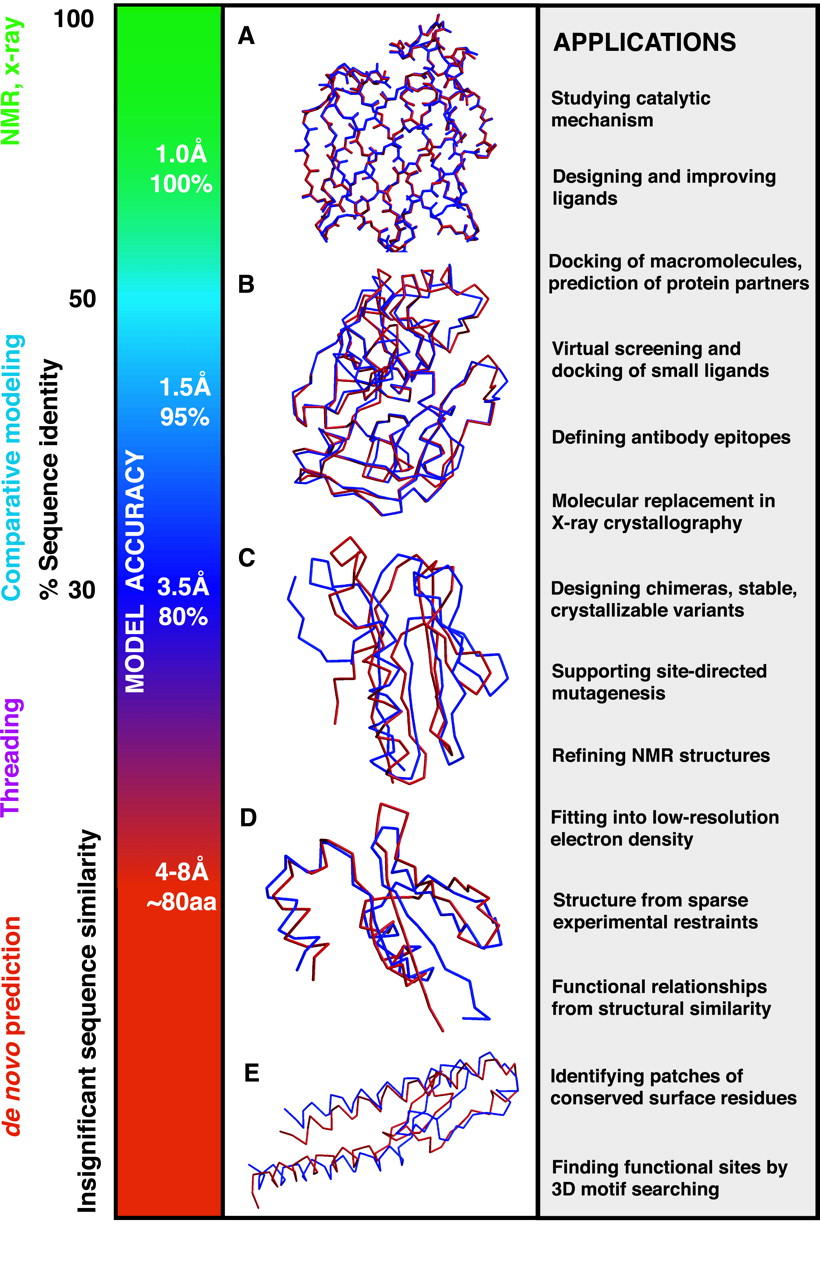
\includegraphics[width = 0.8\textwidth]{figs/sali.jpeg}
\caption{Precisión y aplicación de los modelos de estructura de proteínas (en 2001).}
\end{figure}

Un gran poder conlleva una gran responsabilidad. El uso de modelos conlleva una precaución y una necesidad de validación experimental. Sin embargo, conocer las limitaciones de nuestro modelo es necesario para un uso realista del mismo; y los límites vienen definidos por la calidad del modelo.

La precisión de un modelo comparativo está relacionada con el porcentaje de identidad de secuencia en el que se basa. Los modelos comparativos de alta precisión pueden tener un error cuadrático medio (RMS) de aproximadamente 1-2 $\AA$ para los átomos de la cadena principal, lo que es comparable a la precisión de una estructura de resonancia magnética nuclear (RMN) o una estructura de rayos X. Estos modelos pueden utilizarse para estudios funcionales y la predicción de socios de proteínas, incluidos fármacos u otras proteínas que trabajen en el mismo proceso. Además, para algunos estudios detallados, sería conveniente refinar su modelo mediante Dinámica Molecular y métodos afines hacia una estructura similar a la nativa. 

Por el contrario, los modelos comparativos de baja precisión se basan en una identidad de secuencia inferior al 20-30\%, lo que dificulta la capacidad de modelado y la precisión. Algunos de estos modelos pueden utilizarse con fines de ingeniería de proteínas o para predecir la función de secuencias huérfanas basándose en el pliegue de la proteína (utilizando Dali o Foldseek).
